\chapter{Design}
\section{Systemübersicht}
In der folgenden Abbildung ist das System auf hoher Abstraktionsstufe zu sehen. Die Applikation ist über einen Web Browser bedienbar. Auf dem Management Server werden verschiedenstartige IoT Devices verwaltet. Der Management Server kommuniziert über TCP/IP mit den Devices. 
\begin{figure}[H]
\centering
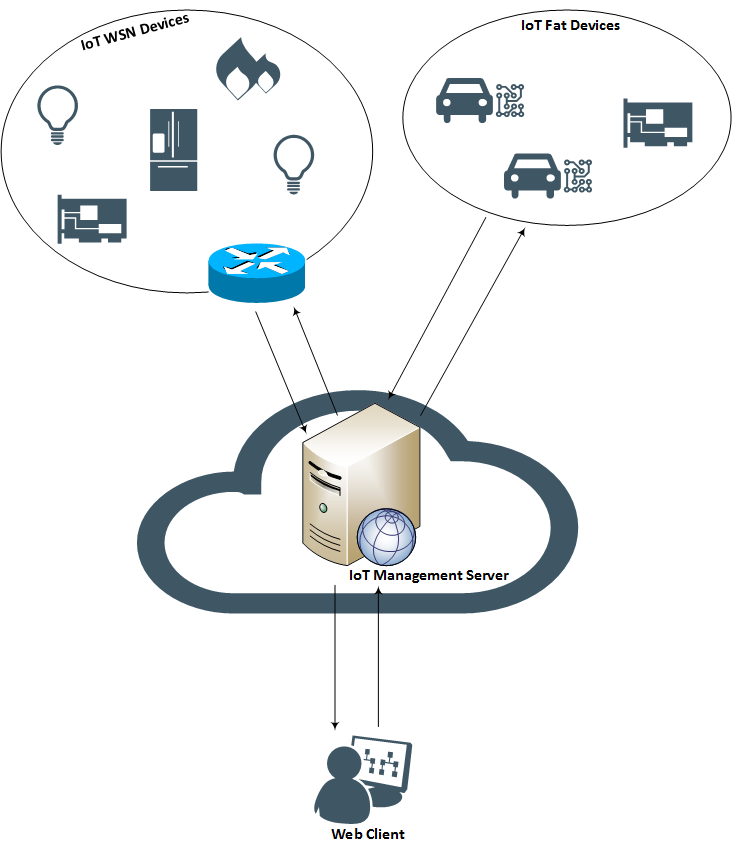
\includegraphics[scale=0.6]{images/systemuebersicht.png}
\caption{Systemübersicht}
\end{figure}
Der User kann seine IoT Devices entweder manuell erfassen, oder über ein Discovery ins System aufnehmen. Sobald ein Device im System ist, können hardware- und konfigurationsspezifische Parameter ausgelesen werden. Gemäss Use Case Analyse sind auch der Austausch von Dateien und das Absetzen von Kommandos vorgesehen. 
\newpage

\begin{landscape}
\section{Klassenstruktur}
\subsection{Klassendiagramm}
\begin{figure}[H]
\centering
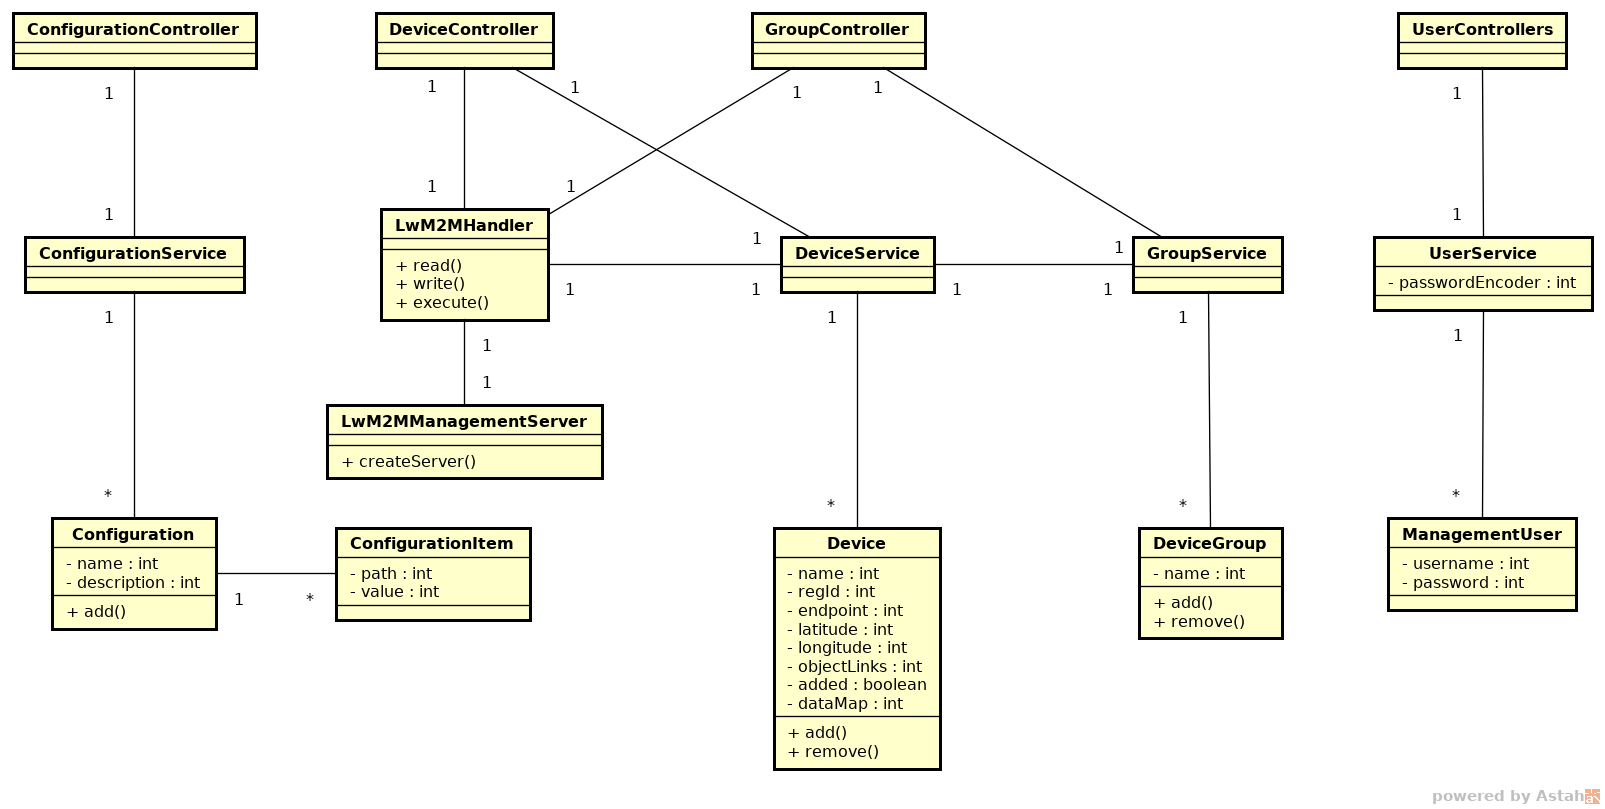
\includegraphics[width=1\textwidth]{images/domainmodel.png}
\caption{Klassendiagramm}
\end{figure}
\end{landscape}
\subsection{Klassenbeschreibungen}
\subsubsection{Connect}
Die Connect-Klasse ist für die Verbindung zu den Geräten zuständig. Sie behandelt die Authentisierung und stellt die Verbindung den anderen Klassen bereit. Dies ist eine zentrale Klassen, welche bei vielen Tätigkeiten benötigt wird.
\begin{table}[H]
\centering
    \begin{tabular}{@{}l p{14.1cm} @{}}\toprule    
    {Eigenschaft} & {Beschreibung}\\ \midrule
    connect() & Die Connect Methode, welche die Verbindung zu einem Device aufbaut.\\
    \bottomrule
    \end{tabular}
\end{table}

\subsubsection{Reader}
Mit dem Reader werden die Daten von den Devices abgefragt. Je nach Device wird eine andere Implementation der Read-Funktion bereitgestellt, damit alle gewünschten Protokolle unterstützt werden.
\noindent \begin{table}[H]
\centering
    \begin{tabular}{@{}l p{14.1cm} @{}}\toprule    
    {Eigenschaft} & {Beschreibung}\\ \midrule      
    read() & Read-Methode, welche die Daten vom gewünschten Device ausliest.\\
    \bottomrule
    \end{tabular}
\end{table}

\subsubsection{Writer}
Die Writer-Klasse schreibt die Kommandos und gewünschten Dateien zu einem Device. Diese Klasse wird für das Updaten, Konfig schreiben, so wie andere Parameter verwendet. Je nach Protokoll gibt es einen spezielle Implementation der Write-Klasse.
\noindent \begin{table}[H]
\centering
    \begin{tabular}{@{}l p{14.1cm} @{}}\toprule    
    {Eigenschaft} & {Beschreibung}\\ \midrule      
    write() & Die write-Methode schickt die gewünschten Daten zum Device. \\
    \bottomrule
    \end{tabular}
\end{table}


\subsubsection{Listener}
Dies ist die Discovery-Klasse. Mit der Listener-Klasse hören wir auf Geräte aus dem Netzwerk und falls welche Vorhanden sind, werden diese in der Datenbank eingefügt. Für die verschiedenen Protokolle gibt es verschiedene Implementationen
\begin{table}[H]
\centering
    \begin{tabular}{@{}l p{14.1cm} @{}}\toprule    
    {Eigenschaft} & {Beschreibung}\\ \midrule
    listen() &  Die Methode nach dem Starten über längere Zeit auf Device-Anfragen und speichert diese.\\
    \bottomrule
    \end{tabular}
\end{table}



\subsubsection{FileHandler}
Der FileHandler ist für den Up- und Download zuständig. Er nimmt alle Dateien entgegen und speichert diese auf dem Server ab. Oder er holt eine Datei vom Server und lädt diese herunter, damit man sie mit dem Writer auf ein Device schicken kann.
\begin{table}[H]
\centering
    \begin{tabular}{@{}l p{14.1cm} @{}}\toprule    
    {Eigenschaft} & {Beschreibung}\\ \midrule 
    upload() & Mit dem Upload wird eine Datei vom Filesystem auf das Managementtool geladen. \\
    download() & Durch den download, kann eine Datei vom Managementtool heruntergeladen werden. \\
    \bottomrule
    \end{tabular}
\end{table}

\subsubsection{Device}
Device ist eine Datenklasse, welche alle Angaben eines Devices speichert. Jedes Device wird so in ein Objekt gespeichert.
\begin{table}[H]
\centering
    \begin{tabular}{@{}l p{14.1cm} @{}}\toprule    
    {Eigenschaft} & {Beschreibung}\\ \midrule      
    name & Gerätenamen \\
    authType & Authentifikationstyp wie zum Beispiel Passwort oder Zertifikat  \\
    ipv4 &  IPv4-Adresse\\
    ipv6 &  IPv6-Adresse\\
    type &  Gerätetyp\\
    vendor & Gerätehersteller \\
    software & Software \\
	location &  Standortangaben des Devices\\    
    \bottomrule
    \end{tabular}
\end{table}

\subsubsection{DeviceGroup}
Durch die DeviceGroup-Klasse wird das Composite-Pattern umgesetzt. So können die Geräte individuell verschachtelt werden.
\begin{table}[H]
\centering
    \begin{tabular}{@{}l p{14.1cm} @{}}\toprule    
    {Eigenschaft} & {Beschreibung}\\ \midrule      
    name & Device Gruppen Namen\\
    description & Beschreibung der Device Gruppe \\
    \bottomrule
    \end{tabular}
\end{table}

\subsubsection{Credential}
Credential-Klasse für die Devices. Durch diese Datenklasse werden alle Usernamen/Passwort kombinationen gehashed abgespeichert. Zusätzlich werden auch die jeweiligen Zertifikate hinterlegt.
\begin{table}[H]
\centering
    \begin{tabular}{@{}l p{14.1cm} @{}}\toprule    
    {Eigenschaft} & {Beschreibung}\\ \midrule      
    username & Benutzername des Devices \\
    password & Devicepassword als Hash\\
    certificate & Zertifikat als Datenblob\\
    hash() & Hashmethode, damit die Passwörter nicht im Klartext gespeichert werden\\
    \bottomrule
    \end{tabular}
\end{table}

\subsubsection{Type}
Die Type-Klasse bestimmt die Verbindungsmethode, sowie das benutzte Protokoll. Diese werden pro Device erfasst.
\begin{table}[H]
\centering
    \begin{tabular}{@{}l p{14.1cm} @{}}\toprule    
    {Eigenschaft} & {Beschreibung}\\ \midrule      
    name & Name des Types \\
    connectionType & Typ der Verbindung, wie zum Beispiel Passwort oder Zertifikat\\
    protocoll & Verwendetes Verbindungsprotokoll\\
    \bottomrule
    \end{tabular}
\end{table}

\subsubsection{Command}
Mit der Command-Klasse werden alle benötigten Kommandos, wie zum Beispiel "Shutdown" usw. erfasst.
\begin{table}[H]
\centering
    \begin{tabular}{@{}l p{14.1cm} @{}}\toprule    
    {Eigenschaft} & {Beschreibung}\\ \midrule      
    command & Device-Kommando\\
    \bottomrule
    \end{tabular}
\end{table}


\subsubsection{File}
Das Interface File, bestimmt die Methoden und Variablen, welche die Vererbten Klassen implementieren müssen.
\begin{table}[H]
\centering
    \begin{tabular}{@{}l p{14.1cm} @{}}\toprule    
    {Eigenschaft} & {Beschreibung}\\ \midrule      
    name & Name der abgelegten Datei\\
    date & Datum\\ 
    Version & Versionsstand der Software oder der Konfigurationsdatei\\
    \bottomrule
    \end{tabular}
\end{table}


\subsubsection{ConfigFile}
Die ConfigFile-Klasse ist die Datenklasse für alle Konfigurationsdateien, damit diese in einer Datenbank angepassten Form gespeichert werden können. \begin{table}[H]
\centering
    \begin{tabular}{@{}l p{14.1cm} @{}}\toprule    
    {Eigenschaft} & {Beschreibung}\\ \midrule      
    - & -\\
    \bottomrule
    \end{tabular}
\end{table}



\subsubsection{SoftwareFile}
Diese Datenklasse ist das Objekt für eine Softwaredatei. So kann die Datei in der Datenbank erfasst werden.
\begin{table}[H]
\centering
    \begin{tabular}{@{}l p{14.1cm} @{}}\toprule    
    {Eigenschaft} & {Beschreibung}\\ \midrule      
    - & -\\
    \bottomrule
    \end{tabular}
\end{table}



\subsubsection{CertificateFile}
Zertifikatdatei-Datenklasse. Mit dieser Klasse werden Zertifikate in Objekte umgewandelt, damit man sie in der Datenbank abspeichern kann.
\begin{table}[H]
\centering
    \begin{tabular}{@{}l p{14.1cm} @{}}\toprule    
    {Eigenschaft} & {Beschreibung}\\ \midrule      
    - & -\\
    \bottomrule
    \end{tabular}
\end{table}


\section{Logische Architektur}
\begin{figure} [H]
	\begin{center}
	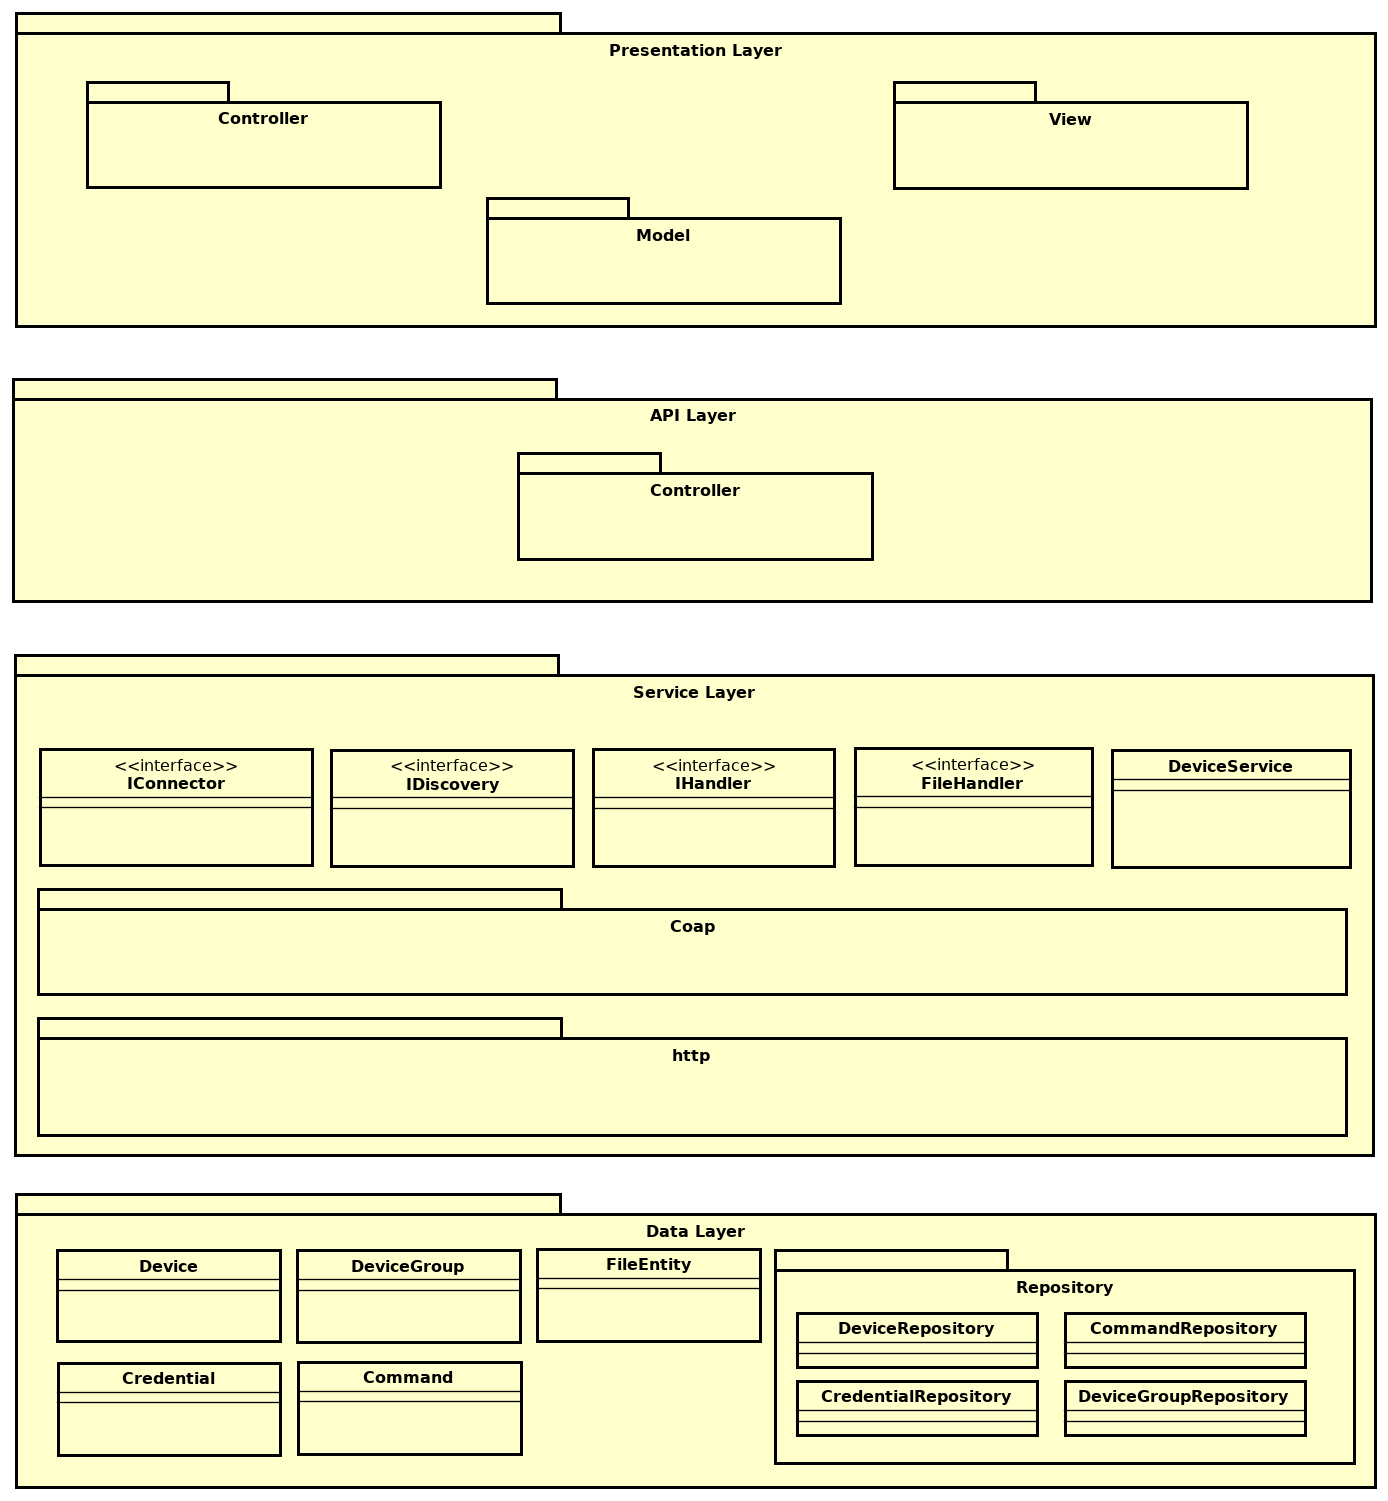
\includegraphics[width=0.90\textwidth]{images/architektur.png}
	\caption{Logische Architektur}
	\end{center}
\end{figure}


\subsection{Presentation-Layer}
Im Presentation-Layer wird das MVC-Pattern umsetzt. Dazu wird ein Controller, eine View sowie ein Model Package implementiert, welche alle Anfragen bearbeiten und anzeigen.
\subsubsection{Packagestruktur}
\begin{table}[H]
\centering
    \begin{tabular}{@{}l p{14.1cm} @{}}\toprule    
    {Packagename} & {Beschreibung}\\ \midrule
    Controller & Der Controller verwaltet alle Anfragen der View und bearbeitet das Model dementsprechend.\\       
    View & Die View bekommt von dem Model die Daten und Renderd dazu die jeweiligen Anzeigen. \\
    Model & Im Model werden alle Daten gehalten, welche die View anzeigt. Nur der Controller hat direkten Zugriff auf diese Daten. \\
    \bottomrule
    \end{tabular}
\end{table}
\subsubsection{Schnittstellen}
Der Presentation-Layer hat direkten Zugriff auf den Service-Layer. Bis jetzt besteht noch keine weitere Schnittstelle.


\subsection{Service-Layer}
Der Service-Layer beinhaltet alle Backend Klassen, welche für die Verarbeitung der Daten zuständig ist. Hier werden alle Devices erfasst, verbunden und verwaltet.
\subsubsection{Klassenstruktur}
\begin{table}[H]
\centering
    \begin{tabular}{@{}l p{11cm} @{}}\toprule    
    {Klassenname} & {Beschreibung}\\ \midrule
    Connect & Die Verbindungsklasse des Servicelayer stellt alle Verbindungen zu den Devices auf.  \\       
     Reader & Alle Daten von den jeweiligen Devices werden von der Reader-Klasse gelesen und an den Data-Layer weitergegeben.  \\       
     Writer &  Der Writer schreibt die gewünschten Daten auf ein Device und aktualisiert die Daten im Data-Layer \\       
     Listener &  Der Listener horcht auf neue Devices und erfasst diese laufend auf dem Data-Layer \\       
     FileHandler &  Mit dem FileHandler werden die Dateiobjekte auf dem Data-Layer erstellt und abgespeichert. \\       
    \bottomrule
    \end{tabular}
\end{table}
\subsubsection{Schnittstellen}
Der Service-Layer hat eine Schnittstelle zum Data-Layer. Durch den Service-Layer werden die Datenobjekte erstellt, bearbeitet und ausgewertet. Der Presentation-Layer muss immer über den Service-Layer, um eine saubere Abtrennung der Schichten zu gewährleisten.

\subsection{Data-Layer}
Der Data-Layer beinhaltet alle Datenobjekte, welche vom laufenden Programm benötigt werden. Diese werden von hier in die Datenbank geschrieben.
\subsubsection{Klassenstruktur}
\begin{table}[H]
\centering
    \begin{tabular}{@{}l p{11cm} @{}}\toprule    
    {Klassenname} & {Beschreibung}\\ \midrule
    Device & Device ist eine Datenklasse, welche alle Daten von einem Device beinhaltet.\\
    Credentials & Alle Zugriffsdaten der Devices sind in der Credentials-Klasse definiert. \\
    Type & Type beinhaltet die Typendefinition, welche den einzelnen Devices zugeordnet werden. \\
    DeviceGroup & In der Datenklasse DeviceGroup, werden alle Gruppen verwaltet, damit das Composite-Pattern umgesetzt werden kann.\\
    Command & Alle Kommandos werden zentral in der Command-Datenklasse gespeichert.\\
    FileEntitiy & In FileEntitiy wird das Grundgerüst für alle Dateien erstellt, damit diese in einer geeigneten Form in der Datenbank abgespeichert werden können.\\ 
    \bottomrule
    \end{tabular}
\end{table}
\subsubsection{Schnittstellen}
Der Data-Layer hat eine Schnittstelle zu der Datenbank.

\section{Architekturentscheidungen}
In diesem Kapitel werden alle Architekturentscheidungen aufgelistet, welche das Front-End, Back-End, sowie die Datenbank betreffen
\subsection{Front-End}
%alternative Bootstrap, angularjs, react, hardcoded
\begin{longtable}{| p{4cm} | p{11.7cm} |}
 \hline
  \textbf{Bereich} & 16\\ \hline 
 \textbf{Problemstellung} & l ''Reboot'' oder ''Shutdown'', gesendet.\\ \hline 
 \textbf{Motivation} &  \\ \hline
 \textbf{Alternativen} &  \\ \hline
 \textbf{Entscheidung} &
\end{longtable}

\subsection{Back-End}
%Alernativen Nodejs, Java Sp§ring, asp.net, play
\begin{longtable}{| p{4cm} | p{11.7cm} |}
 \hline
  \textbf{Bereich} & 16\\ \hline 
 \textbf{Problemstellung} & l ''Reboot'' oder ''Shutdown'', gesendet.\\ \hline 
 \textbf{Motivation} &  \\ \hline
 \textbf{Alternativen} &  \\ \hline
 \textbf{Entscheidung} &
\end{longtable}


\subsection{Datenbanktechnologie}
%Alernativen sql, nosql

\begin{longtable}{| p{4cm} | p{11.7cm} |}
 \hline
  \textbf{Bereich} & 16\\ \hline 
 \textbf{Problemstellung} & l ''Reboot'' oder ''Shutdown'', gesendet.\\ \hline 
 \textbf{Motivation} &  \\ \hline
 \textbf{Alternativen} &  \\ \hline
 \textbf{Entscheidung} & 
\end{longtable}

